\section{When does a book amplify? An exact condition}\label{sec:t6}

Transient path risk takes two forms, and the distinction organizes both the theory and the evidence. The first is \emph{peak overshoot}, a response that rises above its direct impact; Theorem~\ref{thm:t6} shows that it requires depth depletion to outweigh impact-weighted reversion. The second is \emph{cumulative amplification}, a summed response $S$ much larger than direct impact; Proposition~\ref{prop:sum} shows that it arises without any depletion whenever reversion is slow relative to impact and momentum. The guard of Section~\ref{sec:guard} bounds the second. The data of Sections~\ref{sec:depth}--\ref{sec:thin} show no peak overshoot in crypto books, even though flow depletes the side it hits on a fixed price grid, and they support the second form in thin books.

\subsection{A book with depletion and refill}
Let $x_t$ be the price displacement, $d_t$ the signed depth imbalance (bid minus ask depth near the mid, relative to total) and $u_t$ signed order flow. Flow moves the price directly and depletes one side of the book, which refills at rate $r$; depth imbalance moves the price:
\begin{align}
x_t &= a\,x_{t-1} + \varphi\,d_{t-1} + \kappa\,u_t, \label{eq:x}\\
d_t &= (1-r)\,d_{t-1} + \varepsilon\,u_t, \label{eq:d}
\end{align}
with $\kappa>0$, $a\in[0,1)$ and $r\in(0,1]$. Write $b=1-r$. With the sign convention $d=(B-A)/(B+A)$, a buy that consumes ask depth raises $d$, so $\varepsilon>0$ means \emph{depletion} of the side that is hit, and $\varphi>0$ means that a bid-heavy book pushes the price up. The impulse response to a unit flow shock at $t=0$ is $h_0=\kappa$ and
\begin{equation}\label{eq:rec}
h_k=a\,h_{k-1}+\varphi\varepsilon\,b^{k-1},\qquad k\ge1.
\end{equation}

\begin{definition}
The book \emph{amplifies} if $\max_kh_k>h_0$: the price keeps moving in the direction of the shock after the shock has passed.
\end{definition}

\subsection{The two-state theorem}

\begin{theorem}[Amplification condition]\label{thm:t6}
In model \eqref{eq:x}--\eqref{eq:d}, the book amplifies if and only if
\[
C_2\equiv\varphi\varepsilon-(1-a)\kappa>0 .
\]
When $C_2\le0$ the response peaks at impact, $\max_kh_k=\kappa$.
\end{theorem}

\begin{proof}
\emph{If.} $h_1-h_0=a\kappa+\varphi\varepsilon-\kappa=C_2>0$.

\emph{Only if.} Suppose $C_2\le0$. If $\varphi\varepsilon<0$, then by \eqref{eq:rec} $h_k=a^k\kappa+\varphi\varepsilon\sum_{j<k}a^{k-1-j}b^j\le a^k\kappa\le\kappa$. If $\varphi\varepsilon\ge0$, let $\Delta_k=h_k-h_{k-1}$. Then $\Delta_1=C_2\le0$ and, from \eqref{eq:rec},
\[
\Delta_{k+1}=a\Delta_k+\varphi\varepsilon(b^{k}-b^{k-1})=a\Delta_k-\varphi\varepsilon\,r\,b^{k-1}\le a\Delta_k .
\]
By induction $\Delta_k\le0$ for all $k$, so $h$ is non-increasing and peaks at $h_0=\kappa$.
\end{proof}

\paragraph{Interpretation.} The left side $\varphi\varepsilon$ is the extra price pressure that a unit of flow creates one period later through the book it leaves behind. The right side $(1-a)\kappa$ is the part of the direct impact that reverts in one period. The book amplifies exactly when the depth channel adds more than mean reversion removes. Refill $r$ does not enter the condition; it governs how long an overshoot lasts.

\begin{proposition}[Shape of the overshoot]\label{prop:shape}
Let $0<a<1$, $0<b<1$ and $a\neq b$. The response is $h_k=Aa^k+Bb^k$ with $B=\varphi\varepsilon/(b-a)$ and $A=\kappa-B$. When the book amplifies, $Aa^k+Bb^k$, viewed as a function of real $k\ge0$, has a single maximum, at
\[
k^*=\frac{\log\bigl(-A\log a/(B\log b)\bigr)}{\log(b/a)},
\]
so the peak lag is $\lfloor k^*\rfloor$ or $\lceil k^*\rceil$ (and is $1$ when $k^*<1$, because $h_1>h_0$), and the cumulative response is $\sum_kh_k=\kappa/(1-a)+\varphi\varepsilon/[(1-a)r]$. Faster refill lowers both the peak and the cumulative response. In the boundary cases, $h_k=\kappa a^k+\varphi\varepsilon\,k\,a^{k-1}$ when $a=b$, and the response peaks at lag 1 when $a=0$ ($h_k=\varphi\varepsilon b^{k-1}$ for $k\ge1$) or $r=1$ ($h_k=a^{k-1}(a\kappa+\varphi\varepsilon)$ for $k\ge1$); the cumulative formula holds in all cases.
\end{proposition}

We verify Theorem~\ref{thm:t6} in 1,995 random parameter draws and the refill comparative static in 565 amplifying draws, with no exceptions. The peak lag lies in the stated bracket in all of 150{,}039 amplifying draws; it is not always the integer nearest to $k^*$, which an earlier version claimed and which fails in 15\% of draws (\texttt{recompute\_audit.py}). Figure~\ref{fig:t6} illustrates the four cases.

\begin{figure}[t]\centering
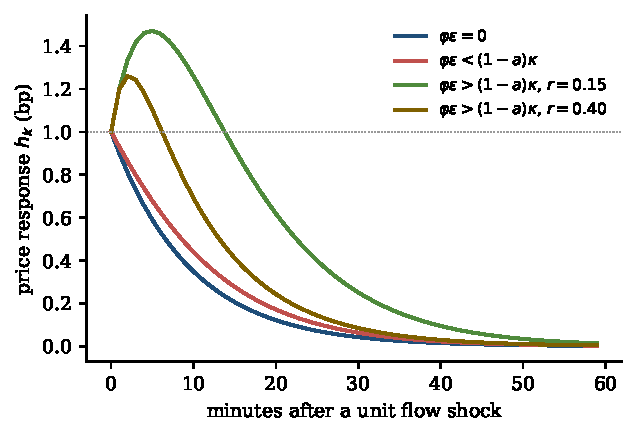
\includegraphics[width=0.6\textwidth]{figs/fig_t6.pdf}
\caption{Illustrative impulse responses of model \eqref{eq:x}--\eqref{eq:d} ($a=0.9$, $\kappa=1$, $\varepsilon=0.1$). The response overshoots only when $\varphi\varepsilon>(1-a)\kappa$; faster refill $r$ lowers the overshoot. Parameters are illustrative, not estimates.}\label{fig:t6}
\end{figure}

\subsection{Momentum traders}

Add momentum traders whose flow $f_t=(1-\eta)f_{t-1}+\eta q\,x_{t-1}$ enters both \eqref{eq:x} and \eqref{eq:d} alongside $u_t$.

\begin{proposition}[One-period amplification margin]\label{prop:t6m}
Let $C_3\equiv\varphi\varepsilon+\kappa^2\eta q-(1-a)\kappa$. Then $h_1-h_0=C_3$, so $C_3>0$ implies that the book amplifies.
\end{proposition}

\begin{proof}
With a unit shock at $t=0$, $x_0=\kappa$, $d_0=\varepsilon$ and $f_1=\eta q\kappa$, so $h_1=a\kappa+\varphi\varepsilon+\kappa^2\eta q$.
\end{proof}

With two slow modes the converse fails, and no condition on the one-period margin is exact. Three results describe what can be said instead.

\begin{theorem}[Momentum alone cannot make a stable book amplify]\label{thm:nomom}
Suppose $\varphi\varepsilon=0$ and $q\ge0$, and the system is stable. Then $h_k\le\kappa\,\rho^k<\kappa$ for every $k\ge1$, where $\rho<1$ is the spectral radius. In particular $C_3<0$.
\end{theorem}

\begin{proof}
Without the depth channel the state $(x_t,f_t)$ evolves by $M=\begin{psmallmatrix}a+\kappa\eta q&\kappa(1-\eta)\\ \eta q&1-\eta\end{psmallmatrix}$, which is entrywise nonnegative, and $h_k=\kappa(M^k)_{11}$. The off-diagonal product is nonnegative, so the eigenvalues are real, and by the Perron--Frobenius theorem $\lambda_2\le m_{11}\le\lambda_1=\rho$. Writing $(M^k)_{11}=c_1\lambda_1^k+c_2\lambda_2^k$ with $c_1=(m_{11}-\lambda_2)/(\lambda_1-\lambda_2)\in[0,1]$ and $c_2=1-c_1$ gives $(M^k)_{11}\le\rho^k$. Since $m_{11}\le\rho<1$, $C_3=\kappa(m_{11}-1)<0$.
\end{proof}

\begin{theorem}[A sufficient condition for no overshoot]\label{thm:noover}
For any signs of $\varphi$, $\varepsilon$ and $q$, if
\[
\bar C_3\equiv|\varphi\varepsilon|\Bigl(1+\frac{\kappa|q|}{r}\Bigr)+\kappa^2|q|-(1-a)\kappa\;\le\;0,
\]
then $\sup_k|h_k|=\kappa$: the response never exceeds its impact in either direction. When $\varphi\varepsilon\ge0$ and $q\ge0$, $C_3>0\Rightarrow$ amplification $\Rightarrow\bar C_3>0$.
\end{theorem}

\begin{proof}
Suppose $|x_j|\le\kappa$ for $j<k$. Then $|f_j|\le|q|\kappa$ for $j\le k$ and $|d_{k-1}|\le|\varepsilon|\bigl(b^{k-1}+\sum_{j\ge1}b^{k-1-j}|q|\kappa\bigr)\le|\varepsilon|(1+|q|\kappa/r)$, so $|x_k|\le a\kappa+|\varphi\varepsilon|(1+\kappa|q|/r)+\kappa^2|q|\le\kappa$. Induction from $x_0=\kappa$ completes the proof.
\end{proof}

\begin{remark}[Counterexamples to an exact one-period condition]\label{rem:counter}
Between $C_3$ and $\bar C_3$ the sign of $C_3$ does not decide. With $\kappa=1$, $a=0.98526$, $\varphi=0.7409$, $\varepsilon=0.01183$, $r=0.03436$, $\eta=0.5092$ and $q=0.01127$ (all channels reinforcing, $\rho=0.9995$), $C_3=-0.00024$ but the response peaks at lag 60 at $1.092\kappa$. With replenishment ($\varphi=2.614$, $\varepsilon=-0.405$, $a=0.9426$, $r=0.033$, $\eta=0.0016$, $q=0.0785$, $\rho=0.998$), $C_3=-1.11$ yet the response oscillates to $9.2\kappa$ at lag 90. In a search over 400{,}000 parameter draws such cases occur only near the stability boundary or with slow refill and slow momentum.
\end{remark}

\begin{proposition}[Summed response in closed form]\label{prop:sum}
Let $\tilde\kappa=\kappa+\varphi\varepsilon/r$ (long-run impact: direct plus depth) and $m=1-a$ (reversion). In the stable three-state model,
\[
S\equiv\sum_{k\ge0}h_k=\frac{\tilde\kappa}{m-q\tilde\kappa},
\]
and when $\varphi\varepsilon\ge0$ and $q\ge0$ the system is stable only if $m>q\tilde\kappa$. When all $h_k\ge0$, $S$ is the summed absolute response that enters the guard of Section~\ref{sec:guard}.
\end{proposition}

\begin{proof}
$S=e_1^\top(I-M_3)^{-1}(\kappa,\varepsilon,0)^\top$ with $M_3$ the transition matrix of $(x,d,f)$. Direct computation gives $\det(I-M_3)=\eta\,[\,r(m-\kappa q)-\varphi\varepsilon q\,]$ and the stated ratio; the formula matches the simulated sums to a relative error of $7\times10^{-14}$ in 3{,}000 stable draws.
\end{proof}

Cumulative transient risk is long-run impact divided by reversion net of momentum. Two practical consequences follow. First, the statistic that matters for losses is the summed response, which grows without bound as reversion falls to $q\tilde\kappa$, even when no single lag overshoots (Theorem~\ref{thm:nomom}). Second, $C_3$ is best read as a one-period amplification margin: it moves with $m$, $q$ and $\tilde\kappa$ in the same direction as $S$ and is what we estimate in Sections~\ref{sec:depth} and~\ref{sec:thin}. Both statistics are invariant in sign to rescaling flow.

